%label:"art:symplectoAndHamiltonian"
%author:JeffHicks
%name:"Symplectomorphisms and Hamiltonian isotopies "
%type:"article"

In previous definitions, we've presented 
\begin{itemize}
    \item some diffeomorphic spaces (i.e. $T^*T^n$ and $(\CC^*)^n$) which should be considered the same as symplectic manifolds.
    \item some spaces which are diffeomorphic (i.e. $S^2$ and itself) which can be equipped with clearly different symplectic structures (i.e. $\text{vol}_g$ and $\text{vol}_{2g}$).
\end{itemize} 
We now introduce an equivalence relation for symplectic structures on a manifold.
%label:"def:symplectomorphism"
%type:"definition"
%name:"symplectomorphism"


    Let $(X,  \omega)$ and $(X',  \omega')$ be symplectic manifolds,  and $\phi: X\to X' $ be a diffeomorphism. 
    We call $\phi$ a \emph{symplectomorphism} if
    \[\phi^*\omega'=\omega.\]
    Given an embedding $\psi: X\to X'$, we say that $\psi$ is a \emph{symplectic embedding} if 
    \[\psi^*\omega'=\omega\]


One property of the canonical symplectic structure on the cotangent bundle $T^*Q$ is that the symplectomorphism type of $T^*Q$ is only dependent on the diffeomorphism type of $Q$ \cite{da2001lectures}.
Let $f: Q_1\to Q_2$ be a diffeomorphism. 
Define the \emph{lift} of $f$ to be a map $f_\#: T^*Q_1\to T^* Q_2$ defined by
\[f_\#(q,p)=(f(q),  ((df_q)^*)^{-1}p\]
The lift plays well with the tautological 1-form, in the sense that if $\lambda_i$ is the tautological 1-form for $T^*Q_i$, then $(f_\#)^*\lambda_2=\lambda_1$. 
    

A particularly interesting type of symplectomorphism is one which arises as an isotopy. A symplectic isotopy is a smooth 1-parameter family of maps $\phi_t: X\times I\to X$ which for fixed values of $t$ give a symplectomorphism, and start at the identity (in the sense that $\phi_0=\operatorname{id}_X$). 
These are examples of smooth isotopies and so they can equivalently be described as the flow of a time-dependent vector field.
%label:"def:flow"
%type:"definition"
%name:"flow"


    Given a time-dependent vector field $V_t$,  the \emph{flow associated to $V$} is the function $\phi_t: X\times \RR\to X$ which
    \begin{itemize}
        \item for all $t$, $\phi_t:X\to X$ is a diffeomorphisms and;
        \item is the identity at time 0 so that $\phi_0=\operatorname{id}_M$ and;
        \item generates the vector field $V_t$ in the sense that 
            \[(V_t)_p:=\frac{d}{ds}\phi_s(\phi^{-1}_t(p))|_{s=t}.\]
    \end{itemize}
    We say that \emph{$ V_t$ is the infinitesimal generator} associated to $\phi_t$. 


There is an equivalence between vector fields and flows.
%label:"thm:existenceOfFlow"
%type:"theorem"
%name:"existence of flows"


    On compact manifolds, every time-dependent vector field has a well defined flow. 


One can check that a smooth isotopy $\phi_t$ is a symplectic isotopy by verifying that the symplectic form is preserved by the infinitesimal generator $V_t$.
This yields an easy to check criterion.
%label:"prp:exactsymplectichamiltonian"
%name:"Description of symplectic flows"
%type:"proposition"
%name:"exactnessOfIsotopy"


    $\phi_t$ is a symplectic isotopy if and only if its infinitesimal generator $V_t$ satisfies 
    \[d(\iota_{V_t}\omega)=0.\]


\begin{proof}
    We prove the forward direction, using that $\phi^*_t\omega=\omega$ for all $t$.
    By taking the derivative with respect to $t$ of both sides, we obtain:
\begin{align*}
    0=&\frac{d}{dt}\phi^*\omega
    =\phi^*_t\mathcal L_{V_t}\omega
\end{align*}
Since $\phi$ is a diffeomorphism,  this is equivalent to the vanishing of $\mathcal L_{V_t}\omega$, 
\begin{align*}
 0=& \mathcal L_{V_t}\omega
\end{align*}
Applying Cartan's formula, and using that $\omega$ is closed,
\begin{align*}
0=&d(\iota_{V_t}\omega)+ \iota_{V_t}(d\omega)=d(\iota_{V_t}\omega).
\end{align*}
This means that $\iota_{V_t}\omega$ is closed.
\end{proof}
One could ask for the stronger condition of exactness for the 1-form $\iota_{V_t}\omega$.
In this case, we can describe vector field $V_t$ by a function on $X$. 
%label:"hamiltonianVectorField"
%type:"definition"
%name:"HamiltonianVectorField"


Let $(X,  \omega)$ be a symplectic manifold, and  $H: X\to \RR$ is a smooth function. The \emph{Hamiltonian vector field of $H$} is the unique vector field $V_H$ such that $dH=\iota_{V_H}\omega$.


The uniqueness of this vector field arises from the non-degeneracy of the symplectic form $\omega$.
This additionally means that to every exact symplectic isotopy we can associate a generating Hamiltonian function.
The Hamiltonian isotopies give a large set of easy-to-describe symplectic isotopies, and the relation between Hamiltonian isotopies and all symplectic isotopies has a nice interpretation in terms of the topology of $X$. 
\begin{corollary}
    If $H^1(X,  \RR)=0$,  then every symplectic isotopy is Hamiltonian. 
\end{corollary}
%label:"exm:hamiltonsEquations"
%type:"example"
%name:"Hamilton's Equations"


    Suppose that we are working in $\RR^{2n}=(q_1,  \ldots , q_n,p_1,  \ldots p_n)  $,  equipped with the standard symplectic form $\omega= \sum_{i=1}^n dp_i \wedge dq_i$.
    We can compute the Hamiltonian vector field for $H: \RR^{2n}\to \RR$,  in local coordinates as  \[V_H=\sum_{k=1}^n \left(a_k \partial_{q_k}+b_k \partial_{p_k}\right)\] where the functions $a_k$ and $b_k$ are given by the formulas
\begin{align*}
    \frac{\partial p_k}{\partial H}=-b_k & & \frac{\partial q_k}{\partial H}=a_k.
    \end{align*}


A notable feature of Hamiltonian flow $V_H$ is that it preserves the level sets of $H$, as 
\[V_H(H)=dH(V_H)=\omega(V_H, V_H)=0.\]
%label:"exm:sphereRotation"
%type:"example"
%name:"rotation of Sphere"


    Consider $S^2=\{(x_0, x_1, x_2)\;|\;x_0^2+x_1^2+x_2^2=1\}$  equipped with the symplectic form agreeing with the standard metric induced from $\RR^3$.
    Take the Hamiltonian 
    \begin{align*}
        H:S^2\to&\RR\\
        (x_0,x_1,x_2)\mapsto& x_2
    \end{align*}
    as drawn in \cref{fig:hamiltonianOnSphere}.
    Since Hamiltonian flow preserves the level sets of $H$, we know that the latitudinal slices are orbits under the action of the Hamiltonian flow. 
    To show that the Hamiltonian flow uniformly rotates the sphere, consider the map  $\phi:S^2\setminus\{(0,0,1), (0,0,-1)\}\into S^1\times \RR\subset \RR^3$, where $S^1\times \RR=\{(x_0, x_1, x_2)\;|\; x_0^2+x_1^2=1\}$, and the embedding is given by the latitudinal projection.
    This projection (the \emph{Gall-Peters} map projection) is area-preserving, and so $\phi$ is a symplectic embedding.
    In these new coordinates, $\omega=d\theta\wedge dx_2$ and $H=x_2$. In the Gall-Peters' coordinates,   $V_H=\partial_\theta$. 
    %tag:000X
%label:"fig:hamiltonianOnSphere"
%author:JeffHicks
%name:"rotation of sphere"
%type:"figure"
%parent:exm:sphereRotation
%caption:"The Hamiltonian flow of the standard height function rotates the sphere counterclockwise relative to the north pole"

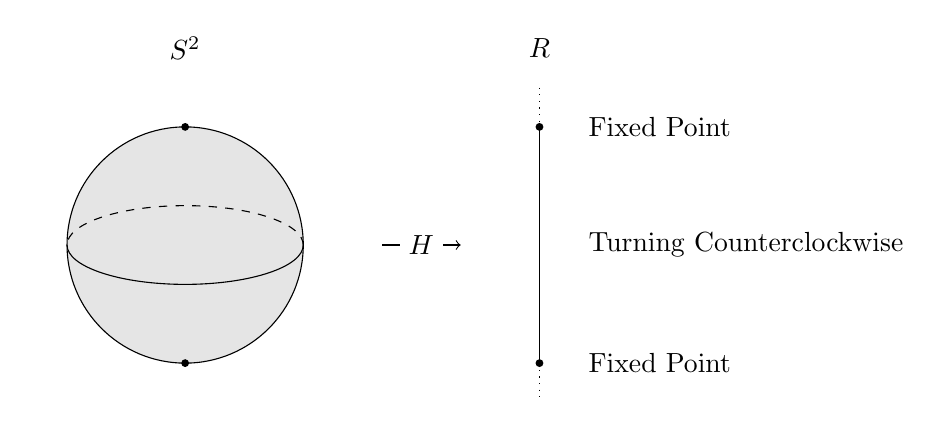
\begin{tikzpicture}
    \draw[fill=gray!20]  (-2,2) ellipse (1.5 and 1.5);
    \begin{scope}[]
    \clip  (-4,2) rectangle (0,3);
    \draw[dashed]  (-2,2) ellipse (1.5 and 0.5);
    \end{scope}
    \begin{scope}[]
    \clip  (-4,2) rectangle (0,1);
    \draw  (-2,2) ellipse (1.5 and 0.5);
    \end{scope}
    
    \draw (2.5,3.5) -- (2.5,0.5);
    \draw[->] (0.5,2) -- (1.5,2);
    \node[fill=white] at (1,2) {$H$};
    \draw[dotted] (2.5,4) -- (2.5,3.5) (2.5,0.5) -- (2.5,0);
    \node at (-2,4.5) {$S^2$};
    \node at (2.5,4.5) {$\mathbb R$};
    \node[right] at (3,3.5) {Fixed Point};
    \node[right] at (3,2) {Turning Counterclockwise};
    \node[right] at (3,0.5) {Fixed Point};
    \node[circle, fill=black, scale=.3] at (-2,3.5) {};
    \node[circle, fill=black, scale=.3] at (-2,0.5) {};
    \node[circle, fill=black, scale=.3] at (2.5,0.5) {};
    \node[circle, fill=black, scale=.3] at (2.5,3.5) {};
    \end{tikzpicture}


The Hamiltonian flow is sometimes called the symplectic gradient. 
In the setting where we have a compatible triple $(X, \omega,g, J)$, the Hamiltonian flow and gradient are related by the almost complex structure. 
%label:"lemma:gradients"
%type:"lemma"
%name:"symplecticGradient"


    Let $(X, \omega, g, J)$ be a compatible triple. Let $H:X\to \RR$ be a Hamiltonian. 
    \[\grad H = J V_H\]


\begin{proof}
    This is a direct computation. On any test vector $v$,
    \begin{align*}
        g(J V_H, v)=\omega(V_H, v)=dH(v)= g(\grad(H), v)
    \end{align*}
    Because $g$ is nondegenerate, $\grad(H)=JV_H$. 
\end{proof}